\begin{figure}[t!]
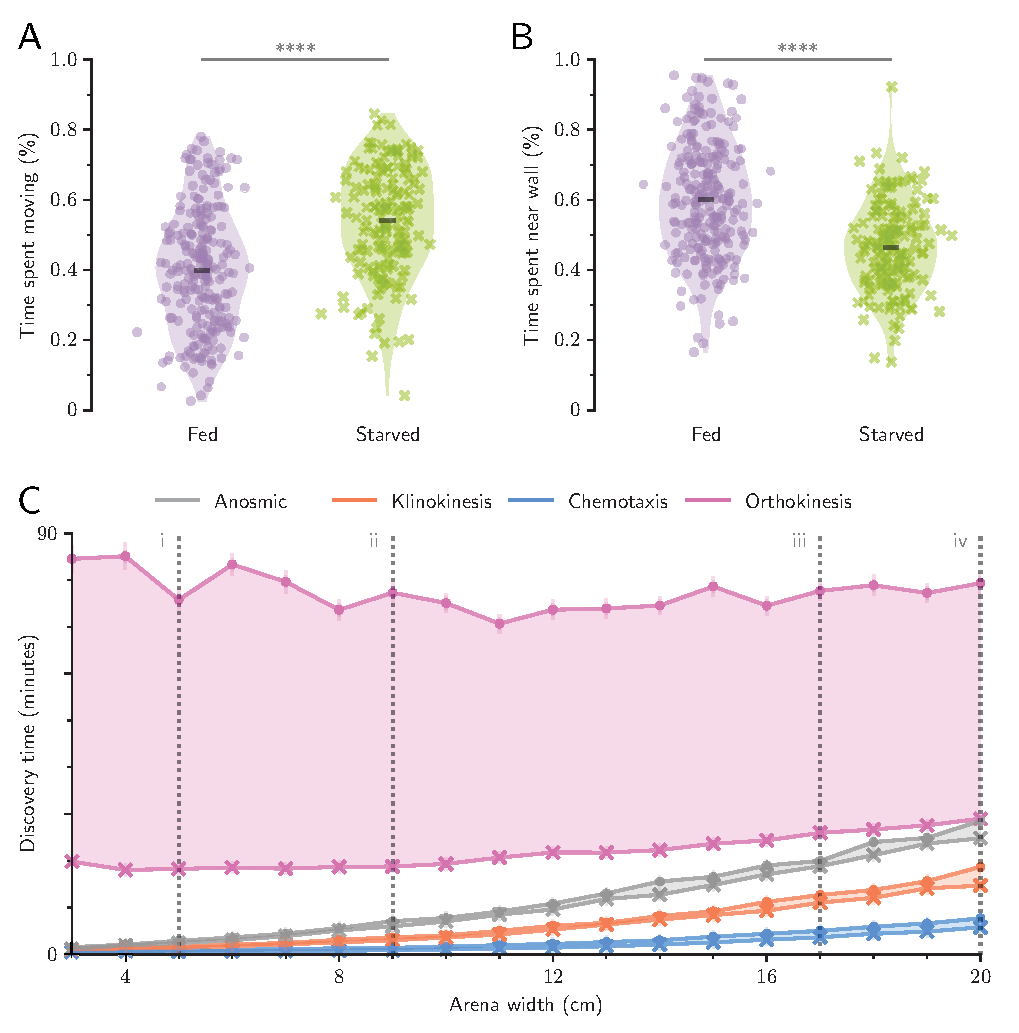
\includegraphics[width=\textwidth]{Figures/images/6.eps}
 \caption{\textbf{ Starved \textit{Ae. aegypti} optimize exploration behavior to increase the probability of finding food.} A: Starved larvae spend significantly more time exploring the arena than fed larvae. B: Starved larvae spend significantly less time within one body length of an arena wall. (A,B) Violin plot. Dots are the means for each individual, and black bar is the mean across all individuals (n>168 per treatment); asterisks denote p<0.0001 (Welch's t-test).  C: Simulated chemokinetic larvae using empirical data from starved animals found the food source consistently faster than the same model using data from fed animals. Shaded regions show difference between fed (X markers) and starved (dots) simulations (mean ${\pm}$ standard error). Dashed grey lines correspond to ecologically relevant habitat sizes described in Table 2. 
}
\end{figure}